{\large \bf
\begin{multicols}{2}
\section*{The Data Plane is continuously evolving.}
\begin{itemize}
\item New scheduling and queue management algorithms are proposed every year.
\item Each wins in its own evaluation under its own workloads.
\item There is a tacit belief in a final answer to these questions.
\end{itemize}

\section*{Yet, there is no silver bullet.}
\subsection*{Different applications care about different things.}
\begin{itemize}
\item Interactive video conferencing apps need both high throughput \& low delay.
\item Bulk transfers care only about high throughput.
\item Web browsers care about minimizing flow completion time (FCT).
\end{itemize}

\subsection*{Applications run different transport protocols.}
\begin{itemize}
\item Some respond to loss, e.g., TCP Cubic, TCP NewReno.
\item Others respond to packet inter-arrival times, e.g., WebRTC, LEDBAT.
\item Others respond to per-packet delay, e.g., TCP Vegas.
\item Yet others respond to both delay and packet loss, e.g., Compound TCP.
\end{itemize}

\subsection*{Applications run in diverse network conditions.}
\begin{itemize}
\item High-speed, low-latency, Data Center networks
\item Low-speed, high-latency, transcontinental links
\item High-speed, high-variability, bufferbloated LTE links
\end{itemize}

\section*{Applications have cyclic preferences}
\subsection*{Workloads:}
\begin{itemize}

\item \textbf{\emph{Bulk}}: 
  \begin{itemize}
  \item Traffic: A single long-running TCP NewReno stream.
  \item Objective: Maximize average throughput.
  \end{itemize}

\item \textbf{\emph{Web}}:
  \begin{itemize}
  \item Traffic: A single on-off TCP NewReno stream.
  \item Objective: Minimize flow completion time at the 99.9th percentile.
  \end{itemize}

\item \textbf{\emph{Interactive}}:
  \begin{itemize}
  \item Traffic: A single long-running TCP NewReno stream.
  \item Objective: Maximize the ratio of average throughput and average
  round-trip delay (``power'').
  \end{itemize}

\end{itemize}


\subsection*{In-network schemes:}
\begin{enumerate}

\item[A)] {\bf CoDel+FCFS}:
  \begin{itemize}
  \item Queue management: CoDel
  \item Scheduling: FCFS
  \end{itemize}

\item[B)] {\bf CoDel+FQ}:
  \begin{itemize}
  \item Queue management: CoDel
  \item Scheduling: Fair Queuing
  \end{itemize}

\item[C)] {\bf Bufferbloat+FQ}:
  \begin{itemize}
  \item Queue management: Don't drop any packets.
  \item Scheduling: Fair Queuing
  \end{itemize}

\end{enumerate}

\subsection*{Visualizing cyclic preferences}
\textbf{None of the below queue-management and scheduling configurations is best. Power is throughput/delay. $A\to B$ indicates that A is better than B.} \\
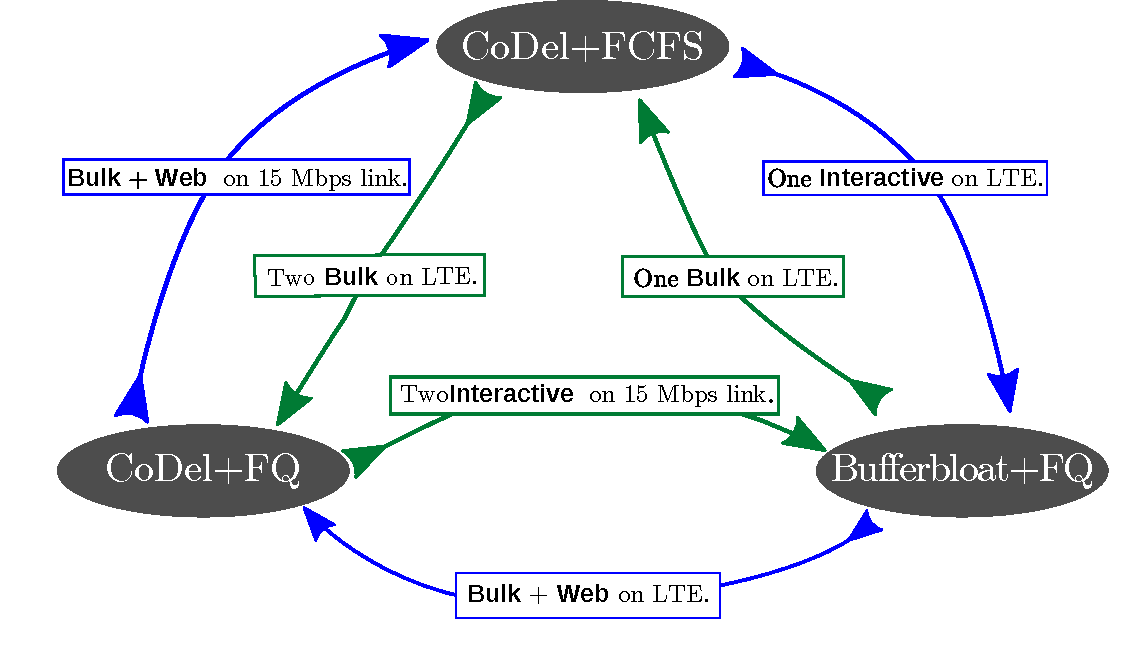
\includegraphics[width=\columnwidth]{fig.pdf}

\section*{Key Findings}
\begin{itemize}
\item Dropping packets on a variable link results in substantial throughput loss.
      \begin{itemize}
      \item Reason: There is an inherent delay-throughput tradeoff, unlike static links.
      \end{itemize} 
 
\item FCFS is preferable to Fair Queuing in some cases.
      \begin{itemize}
      \item Reason: When competeing flows are equally aggressive, they don't need protection from each other.
      \end{itemize}

\item Fair Queuing is required in some cases.
      \begin{itemize}      
      \item Reason: When competing flows are not equally aggressive, they need isolation from each other.
      \end{itemize}

\item Dropping packets hurts Flow Completion Time.
      \begin{itemize}
      \item Reason: Packet drops occur near the end of a flow, preventing DUP ACKs.
      \end{itemize}

\end{itemize}

%\textbf{Detailed results}
%\begin{tabular}{p{0.45\columnwidth}p{12 pt}p{0.45\columnwidth}}

\begin{minipage}{0.45 \columnwidth}
%\centering
CoDel+FCFS beats CoDel+FQ; LTE
\begin{tabular}{| p{6cm} |p{8cm} | }
\hline
Nwk config. & Avg. tpt. \\
\hline
CoDel+FCFS & \cellcolor{green!20} 1.99 Mbps \\
\hline
CoDel+FQ & \cellcolor{red!20} 1.89 Mbps \\
\hline
\end{tabular}
\label{t:cfsbeatscfq}
\end{minipage} & &

\begin{minipage}{0.45 \columnwidth}
CoDel+FQ beats CoDel+FCFS; 15 Mbps
\begin{tabular}{| p{5cm} |p{7.0cm} | p{6cm} | }
\hline
Nwk config. & Bulk Tpt. & Web Tail FCT  \\
\hline
CoDel+FCFS & 9.47 Mbps & \cellcolor{red!20} 22.25 secs \\
\hline
CoDel+FQ & 9.47 Mbps & \cellcolor{green!20} 18.70 secs \\
\hline
\end{tabular}
\label{t:cfqbeatscfs}
%\caption{CoDel+FQ vs.~CoDel+FCFS}
\end{minipage} \\

\end{tabular}
\\
\begin{tabular}{p{0.45\columnwidth}p{12 pt}p{0.45\columnwidth}}

\begin{minipage}{0.45 \columnwidth}
%\centering
Bufferbloat+FQ beats Codel+FQ; LTE
\begin{tabular}{| p{6cm} |p{4.5cm} | p{5.0cm} | }
\hline
Nwk config. & Bulk Tpt. & Web Tail FCT\\
\hline
Bufferbloat+FQ & \cellcolor{green!20} 11.07 Mbps & \cellcolor{green!20} 23 secs \\
\hline
CoDel+FQ & \cellcolor{red!20} 3.86 Mbps & \cellcolor{red!20} 40 secs \\
\hline
\end{tabular}
\label{t:bfqbeatscfq}
\end{minipage} & &

\begin{minipage}{0.45 \columnwidth}
CoDel+FQ beats Bufferbloat+FQ; 15 Mbps
\begin{tabular}{| p{6cm} |p{8cm}| p{6cm}| }
\hline
Nwk config. & Avg. tpt., delay & Power\\
\hline
Bufferbloat+FQ  & 7.47 Mbps, 62000 ms & \cellcolor{red!20} 0.12 $Mbit/s^{2}$ \\
\hline
CoDel+FQ & 6.55 Mbps, 76.5 ms  & \cellcolor{green!20} 85.6 $Mbit/s^{2}$\\
\hline
\end{tabular}
\label{t:cfqbeatsbfq}
%\caption{CoDel+FQ vs.~Bufferbloat+FQ; Power is tpt./delay.}
\end{minipage} \\

\end{tabular}


\begin{tabular}{p{0.45\columnwidth}p{12 pt}p{0.45\columnwidth}}

\begin{minipage}{0.45 \columnwidth}
%\centering
Bufferbloat+FQ beats CoDel+FCFS; LTE
\begin{tabular}{| p{6.0cm} |p{8.0cm} |  }
\hline
Nwk config. & Bulk tpt.  \\
\hline
Bufferbloat+FQ & \cellcolor{green!20} 11.96 Mbps \\
\hline
CoDel+FCFS & \cellcolor{red!20} 4.35 Mbps \\
\hline
\end{tabular}
\label{t:bfqbeatscfs}
\end{minipage} & &

\begin{minipage}{0.45 \columnwidth}
CoDel+FCFS beats Bufferbloat+FQ; LTE
\begin{tabular}{| p{6cm} |p{8.5cm} |p{5.5cm}| }
\hline
Nwk config. & Tpt., delay & Power\\
\hline
Bufferbloat+FQ & 11.96 Mbps, 46000~ms & \cellcolor{red!20} 0.25 $Mbit/s^{2}$\\
\hline
CoDel+FCFS & 4.35 Mbps, 78.2~ms & \cellcolor{green!20}55.62 $Mbit/s^{2}$ \\
\hline
\end{tabular}
\label{t:cfsbeatsbfq}
%\caption{CoDel+FCFS vs.~Bufferbloat+FQ; Power is tpt./delay.}
\end{minipage} \\

\end{tabular}

\section*{The Solution:}
\subsection*{Make the Data Plane more flexible.}
\begin{itemize}
\item There will never be one conclusive queueing and scheduling scheme.
\item Application demands will continue to evolve.
\item Networks supporting these application will evolve as well.
\item The Data Plane should support new queueing and scheduling schemes.
\item Not the same as just picking between multiple existing schemes.
\end{itemize}

\subsection*{But, do so in a controlled manner.}
\begin{itemize}
\item Prevent arbitrary programs from running on the switch.
\item Allow the network operator to determine only queuing and scheduling.
\end{itemize}

\section*{A blueprint for a flexible Data Plane}

\begin{itemize}
\item Standardized interfaces to the rest of the switch

\begin{center}

\begin{tabular}{|l|l|l|}
\hline
\bf Class of primitive & \bf Primitive Name & \bf Description \\
\hline
Utilities & $Now$ & Get current time. \\
\hline
Queue primitives & $Size$ & Get queue length. \\
\hline
Queue primitives & $DropFront$ & Drop packet from head of queue.  \\
\hline
Queue primitives & $DropTail$ & Drop packet from tail of queue. \\
\hline
Queue primitives & $Enqueue$ & Enqueue packet at tail of queue. \\
\hline
Queue primitives & $Dequeue$ & Dequeue packet from head of queue. \\
\hline
Queue primitives & $Transmit$ & Transmit single packet. \\
\hline
Signaling primitives & $LinkReady$ & Link is ready to accept packet. \\
\hline
Signaling primitives & $Arrival$ & New packet just arrived. \\
\hline
Packet primitives & $Timestamp$ & Packet's arrival timestamp. \\
\hline
Packet primitives & $Mark$ & Set ECN bit. \\
\hline
Cross-layer primitives & $LinkRates$ & Get current link rate. \\
\hline
\end{tabular}
\end{center}

\item Add a small amount of reconfigurable logic to the switch.
\item Enforce hard resource limits on the amount of reconfigurable logic.
\item Express queuing/scheduling logic as code in a high-level language.
\end{itemize}

\section*{Example implementation: CoDel}

\begin{itemize}
\item CoDel implementation in SystemVerilog.
\item Synthesized into gate-level netlist using Xilinx's freely available Vivado WebPacket compiler.
\item Block diagram of implementation:
\\
\begin{center}
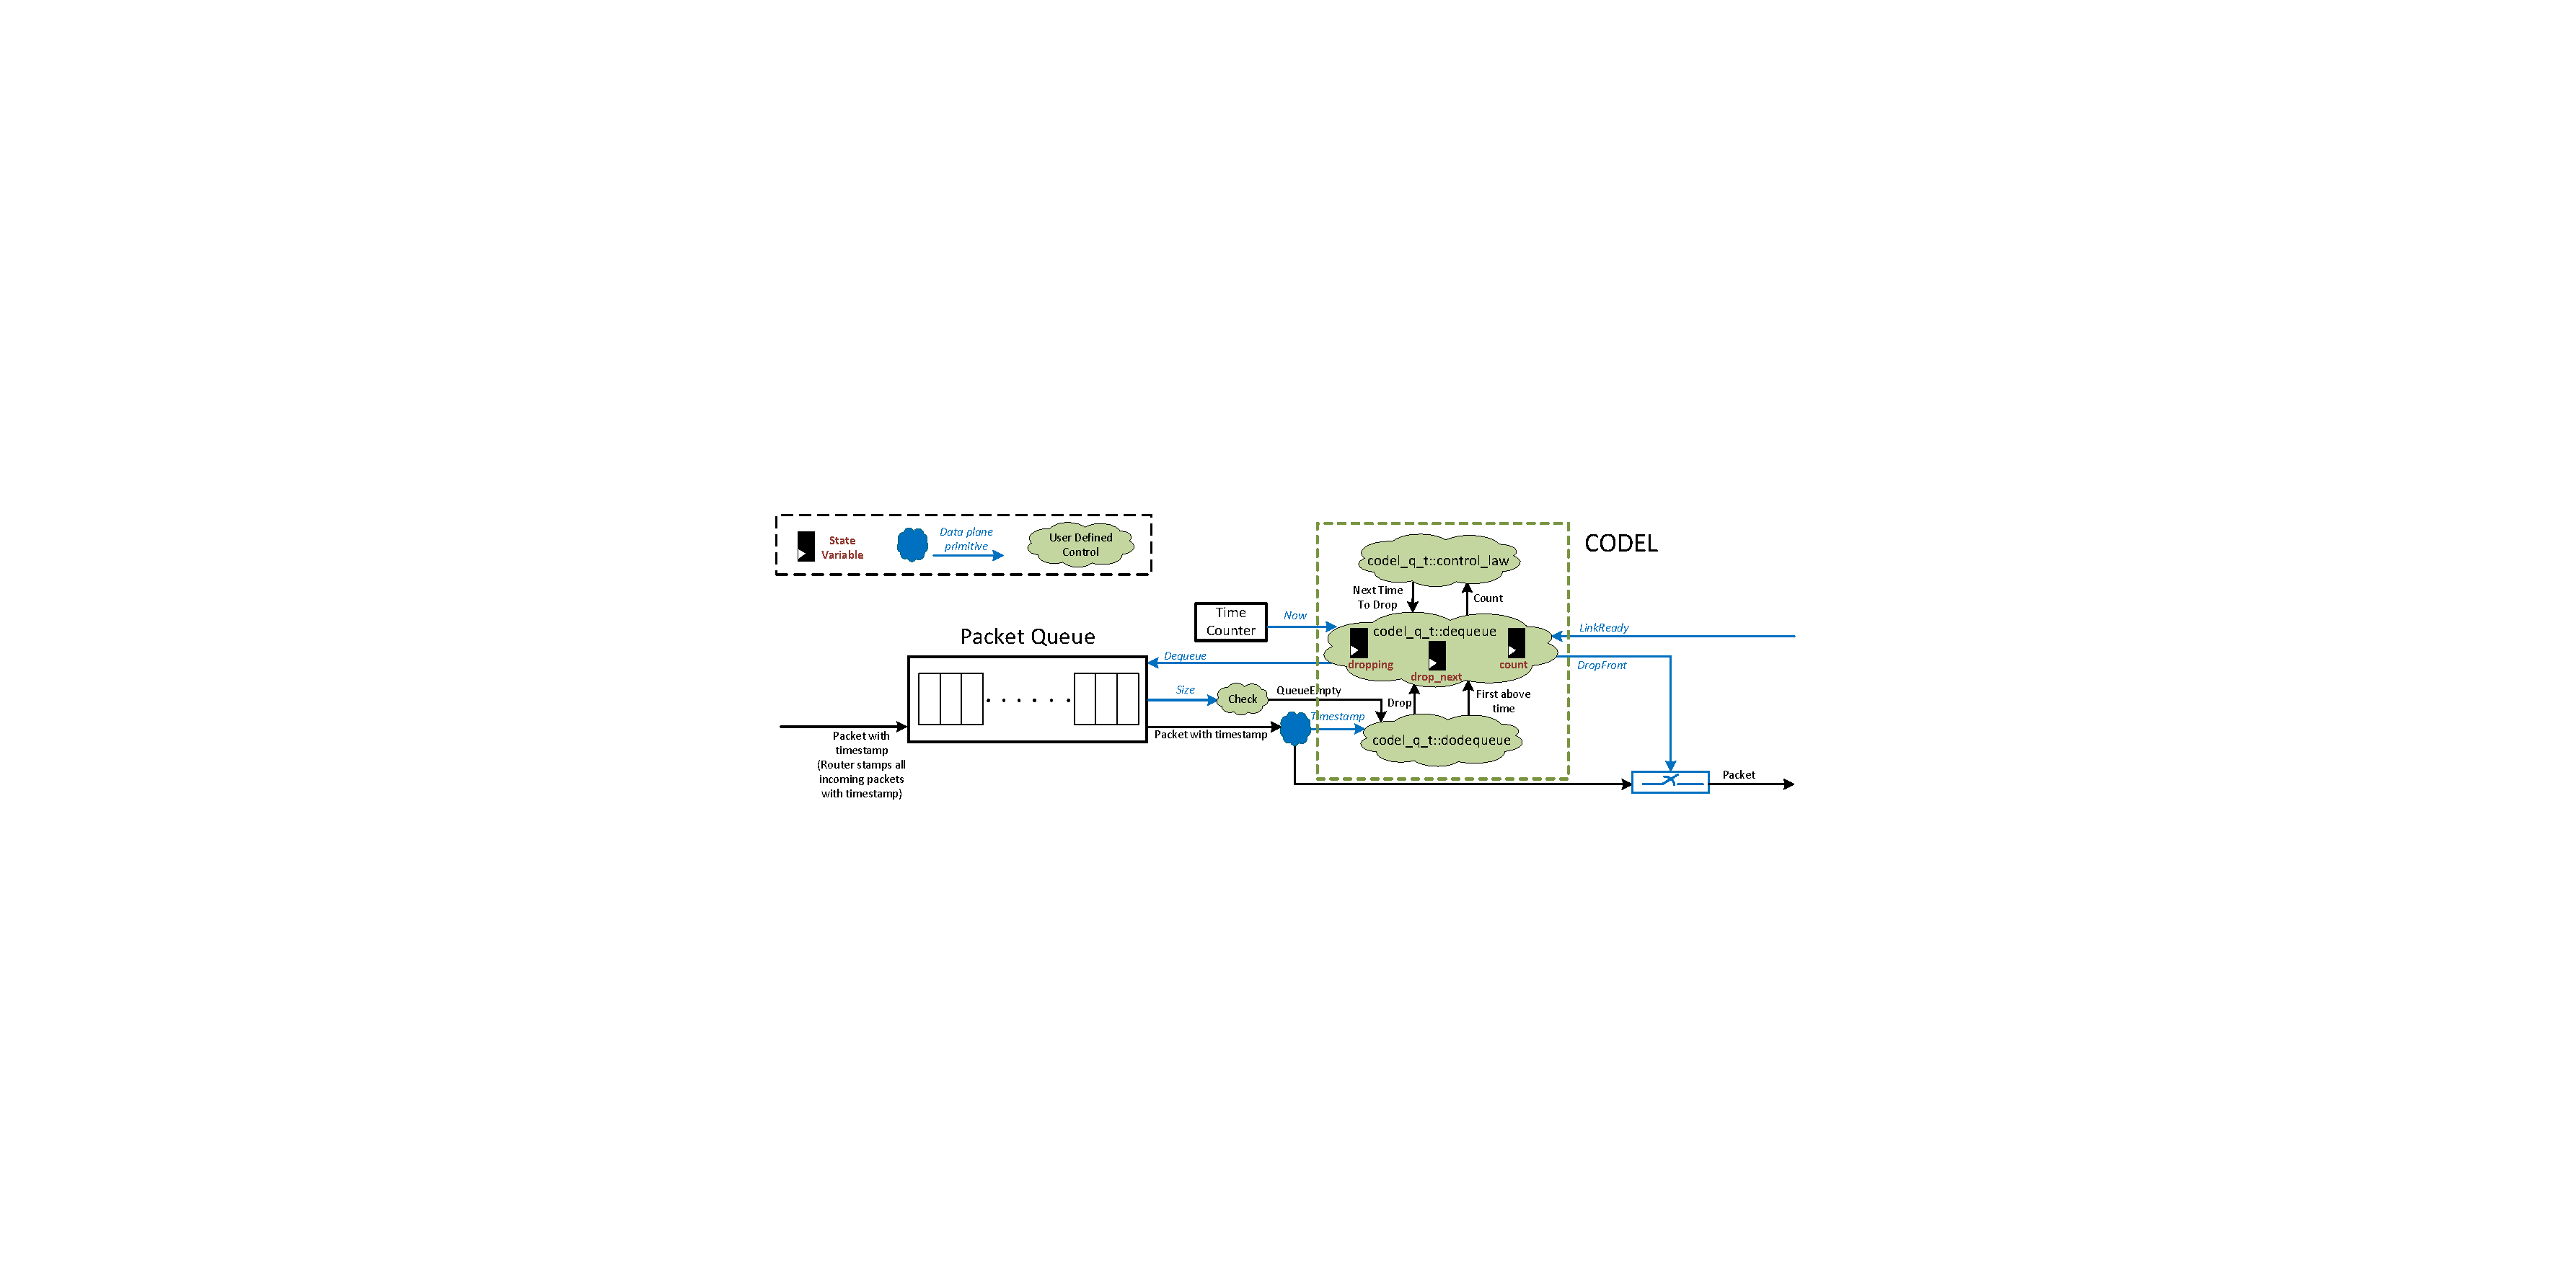
\includegraphics[width=\columnwidth]{codel.pdf}
\end{center}
\item \textbf{CoDel resource utilization on Xilinx Kintex-7:}\\
\begin{center}
\begin{tabular}{|l|l|l|}
\hline
\bf Resource & \bf Usage & \bf Fraction of FPGA \\
\hline Slice logic & 1,257 & 2\% \\
\hline Slice logic dist. & 1,969 & 4\% \\
\hline IO/GTX ports & 27 & 6\% \\
\hline DSP slices & 0 & 0\% \\
\hline Maximum speed & 12.9 $\times 10^6$ pkts/s & N/A \\
\hline
\end{tabular}
\end{center}

\end{itemize}

\section*{Limitations}
\begin{itemize}
\item Cannot express several important network functions:
      \begin{itemize}
      \item ``Deep-packet'' Inspection
      \item Intrusion Detection
      \item Spam Filtering
      \end{itemize}
\item Mechanism for signaling application objectives to the network.
      \begin{itemize}
      \item Could use DiffServ codepoints.
      \item But ASes generally don't honor codepoints from other ASes.
      \item May be a non-issue inside a Data Center.
      \end{itemize}
\item Most switches today have a shared pipeline with demanding requirements.
      \begin{itemize}
      \item Top-of-the-line switches have 64 ports, each running at 10G.
      \item Implies that queueing/scheduling logic should run at 64*10G.
      \item If queue management is enqueue-based, e.g., RED, this problem cannot be fixed by replicating digital logic on each port.
      \end{itemize}
\item Mechanism to map flows onto per-port queues is required for scheduling.
      \begin{itemize}
      \item Also need to decide on the number of such queues.
      \end{itemize}
\item Interoperability
      \begin{itemize}
      \item Across switch vendors.
      \item Across FPGA vendors.
      \end{itemize}
\item Energy and Area overheads.
\end{itemize}

\end{multicols}
}
